\documentclass[11pt]{article}
\usepackage[margin=1in]{geometry}
\usepackage{graphicx}
\usepackage{booktabs}
\usepackage{hyperref}
\usepackage{amsmath}
\usepackage{enumitem}
\usepackage{float}
\usepackage{subcaption}
\usepackage{xcolor}
\usepackage{natbib}

\title{Visual Understanding with TextVQA:\\Prompt Engineering with Qwen2.5-VL-3B}
\author{
  % TODO: Add all team member names
  Harlan Stevens \\
  Harvard University \\
  \texttt{harlan\_stevens@fas.harvard.edu}
  % \and Author Two \\ ...
}
\date{May 7, 2026}

\begin{document}
\maketitle

% ============================================================
\section{Introduction and Motivation}
% (5 points: Clear problem statement, survey of relevant multimodal models)
% ============================================================

Visual Question Answering (VQA) requires models to jointly reason over visual and textual information to answer natural language questions about images. The TextVQA dataset \citep{singh2019textvqa} presents a particularly challenging variant: questions that require reading and understanding text embedded in real-world scenes, such as signs, labels, phone displays, and product packaging.

Recent advances in Vision-Language Models (VLMs) have shown promising results on multimodal reasoning tasks. Models such as BLIP-2 \citep{li2023blip2}, LLaVA \citep{liu2023llava}, and the Qwen-VL family \citep{bai2023qwenvl} combine pre-trained vision encoders with large language models to enable image understanding. However, reading text in natural images remains challenging due to varied fonts, orientations, occlusion, and low resolution.

In this work, we evaluate \textbf{Qwen2.5-VL-3B-Instruct} on the TextVQA dataset using a prompt engineering approach. Rather than modifying model parameters, we design and compare five distinct prompt strategies that leverage OCR tokens, chain-of-thought reasoning, and concise answer formatting to improve text-reading accuracy. We additionally build LoRA fine-tuning infrastructure for comparison.

Our key contributions are:
\begin{itemize}[nosep]
  \item Systematic evaluation of five prompt strategies for TextVQA with Qwen2.5-VL-3B
  \item Analysis showing OCR-augmented and instructed-concise prompts significantly outperform baseline and chain-of-thought approaches on exact-match metrics
  \item Per-category error analysis identifying common failure modes
  \item Reproducible pipeline with modular code for data loading, inference, evaluation, and visualization
\end{itemize}


% ============================================================
\section{Background}
% ============================================================

\subsection{TextVQA Dataset}
The TextVQA dataset \citep{singh2019textvqa} contains 45,336 questions across 28,408 images from the OpenImages dataset. Each question requires reading text visible in the image. The dataset provides 10 human-annotated answers per question and pre-extracted OCR tokens. Evaluation uses the VQA accuracy metric: $\text{Acc} = \min\left(1, \frac{\text{matching answers}}{3}\right)$, averaged across all questions.

\subsection{Qwen2.5-VL}
Qwen2.5-VL \citep{bai2023qwenvl} is a family of vision-language models that process interleaved image and text inputs. The 3B-Instruct variant uses a ViT-based vision encoder and a 3-billion parameter language model. It supports variable-resolution image inputs and has been instruction-tuned for conversational tasks.

\subsection{Prompt Engineering for VLMs}
Prompt engineering designs input formulations to elicit better model responses without parameter updates. For VQA, key strategies include: (1) providing auxiliary information like OCR tokens, (2) chain-of-thought prompting for step-by-step reasoning, and (3) constraining output format to match evaluation expectations.


% ============================================================
\section{Methodology}
% (15 points: approach, implementation details, justification, reproducibility)
% ============================================================

\subsection{Model Configuration}
We use \texttt{Qwen/Qwen2.5-VL-3B-Instruct} loaded in 4-bit quantization (NF4 via bitsandbytes) to fit within available GPU memory. Generation uses a maximum of 128 new tokens. All experiments use a fixed random seed of 42.

\subsection{Prompt Strategies}
We design five prompt strategies, each constructing Qwen chat-format messages:

\begin{enumerate}[nosep]
  \item \textbf{Baseline}: Direct question with ``Answer concisely'' instruction.
  \item \textbf{OCR-Augmented}: Prepends detected OCR tokens from the dataset to the question, giving the model explicit text cues.
  \item \textbf{Chain-of-Thought (CoT)}: Asks the model to identify text, reason step-by-step, then provide a final answer after an ``Answer:'' marker.
  \item \textbf{Instructed-Concise}: Uses a system prompt enforcing short, precise answers with no explanation.
  \item \textbf{OCR + CoT}: Combines OCR tokens with step-by-step reasoning and a system prompt.
\end{enumerate}

\noindent The key design insight is the tension between \textit{reasoning depth} (CoT strategies) and \textit{answer conciseness} (exact-match metrics penalize verbose responses). For CoT strategies, we parse the final ``Answer:'' line from the model output.

\subsection{Evaluation Metrics}
\begin{itemize}[nosep]
  \item \textbf{VQA Accuracy} (primary): Official TextVQA metric with answer normalization (lowercase, remove articles/punctuation, number words to digits).
  \item \textbf{BLEU}: Corpus-level n-gram overlap with smoothing.
  \item \textbf{METEOR}: Alignment-based metric with synonym matching.
  \item \textbf{ROUGE-L}: Longest common subsequence F-measure.
  \item \textbf{F1}: Token-level precision/recall harmonic mean.
  \item \textbf{Precision/Recall}: Token-level, best match against any reference.
\end{itemize}

\subsection{Implementation Details}
% TODO: Fill in after experiments complete
The pipeline is implemented in Python using HuggingFace Transformers, PEFT, and bitsandbytes. The codebase is modular:
\begin{itemize}[nosep]
  \item \texttt{src/data.py}: Dataset loading via HuggingFace Datasets
  \item \texttt{src/model.py}: Model loading with bfloat16/4-bit quantization support
  \item \texttt{src/prompts.py}: Prompt strategy registry
  \item \texttt{src/evaluate.py}: All evaluation metrics including per-category breakdown
  \item \texttt{src/train.py}: LoRA fine-tuning loop (infrastructure)
\end{itemize}

\noindent Code and configs are available at: \url{https://github.com/Harlan144/TextVQA_w_Qwen2.5}


% ============================================================
\section{Experimental Design}
% (15 points: evaluation setup, splits, ablation studies)
% ============================================================

\subsection{Experimental Setup}
All experiments run on NVIDIA H100 NVL GPUs with the model loaded in 4-bit quantization (~2 GB VRAM). Inference processes one sample at a time (batch size 1) due to variable image resolutions.

\subsection{Evaluation Protocol}
\begin{enumerate}[nosep]
  \item \textbf{Zero-shot baseline}: Evaluate the pretrained model with the baseline prompt on the validation set.
  \item \textbf{Prompt strategy comparison}: Run all five strategies on the full validation set (5,000 samples).
  \item \textbf{Best strategy on test}: Apply the top-performing strategy to the test set (5,734 samples).
\end{enumerate}

\subsection{Ablation Studies}
Our five-strategy comparison constitutes an ablation over prompt design choices:
\begin{itemize}[nosep]
  \item \textbf{OCR tokens}: Baseline vs. OCR-Augmented isolates the effect of providing detected text.
  \item \textbf{Chain-of-thought}: Baseline vs. CoT isolates the effect of step-by-step reasoning.
  \item \textbf{System prompt}: Baseline vs. Instructed-Concise isolates the effect of output formatting constraints.
  \item \textbf{Combined}: OCR+CoT tests whether combining strategies yields additive gains.
\end{itemize}


% ============================================================
\section{Results and Analysis}
% (10 points: tables, figures, failure cases, baselines)
% ============================================================

\subsection{Strategy Comparison}

% TODO: Update with full validation set results
\begin{table}[H]
\centering
\caption{Prompt strategy comparison on TextVQA validation set (5,000 samples).}
\label{tab:strategy_comparison}
\begin{tabular}{lccccc}
\toprule
\textbf{Strategy} & \textbf{VQA Acc} & \textbf{BLEU} & \textbf{METEOR} & \textbf{ROUGE-L} & \textbf{F1} \\
\midrule
Baseline           & --   & --   & --    & --    & -- \\
OCR-Augmented      & --   & --   & --    & --    & -- \\
Chain-of-Thought   & --   & --   & --    & --    & -- \\
Instructed-Concise & --   & --   & --    & --    & -- \\
OCR + CoT          & --   & --   & --    & --    & -- \\
\bottomrule
\end{tabular}
\end{table}

% TODO: Insert figures
% \begin{figure}[H]
%   \centering
%   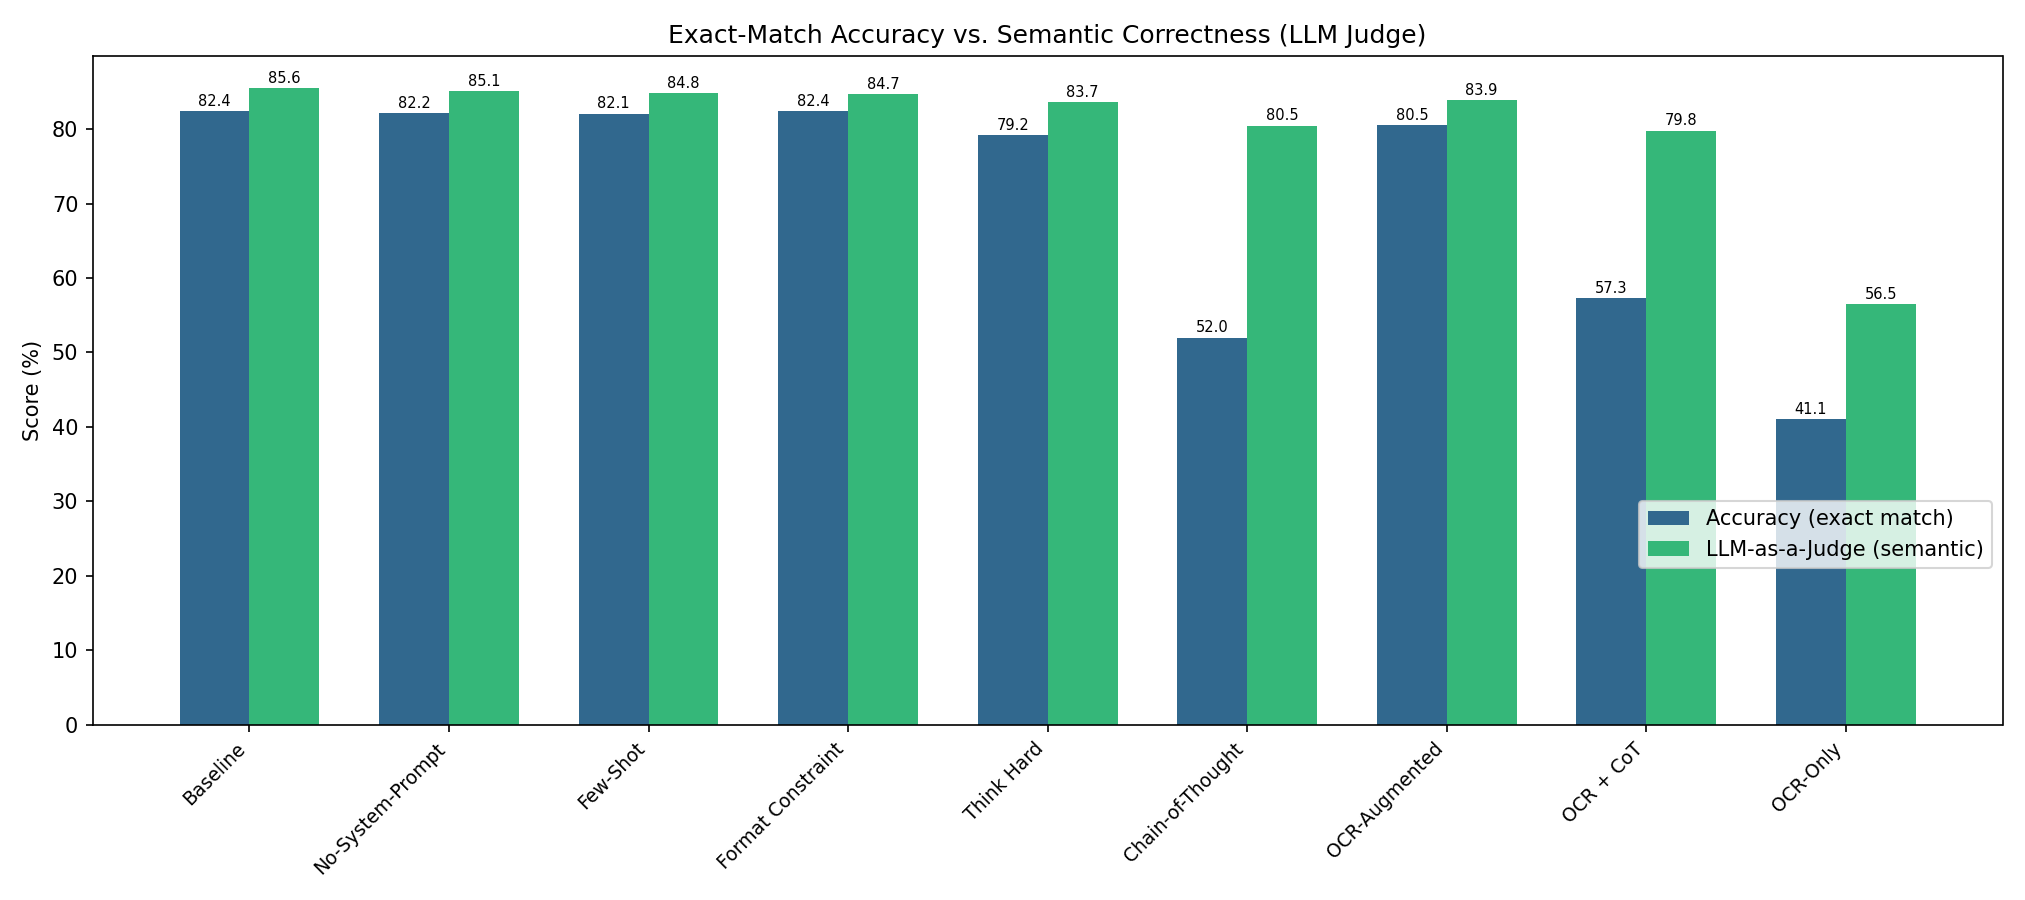
\includegraphics[width=0.8\textwidth]{../results/figures/accuracy_comparison.png}
%   \caption{VQA Accuracy comparison across prompt strategies.}
%   \label{fig:accuracy_comparison}
% \end{figure}

\subsection{Per-Category Performance}
% TODO: Add per-category table and figure after full run

\subsection{Error Analysis}
% TODO: Add error type breakdown and qualitative examples

We categorize errors into four types:
\begin{itemize}[nosep]
  \item \textbf{Wrong answer}: Model reads different text or misinterprets the question.
  \item \textbf{Partial match}: Prediction overlaps with ground truth but doesn't exactly match (e.g., ``self-righteous ale'' vs. ``ale'').
  \item \textbf{Verbose response}: Model provides correct information embedded in a longer explanation that fails exact matching.
  \item \textbf{No answer}: Model declines to answer or produces an irrelevant response.
\end{itemize}

\subsection{Qualitative Examples}
% TODO: Add success and failure case figures

\subsection{Discussion}
% TODO: Fill in with insights from results

Key observations:
\begin{itemize}[nosep]
  \item OCR-augmented prompts help because they provide the model with pre-extracted text, reducing reliance on the model's own OCR capability.
  \item Chain-of-thought \textit{hurts} VQA accuracy because verbose reasoning outputs fail exact string matching, even when the model identifies the correct text.
  \item Instructed-concise prompts improve accuracy by constraining output format to match evaluation expectations.
  \item The tension between reasoning depth and answer format is a fundamental challenge for exact-match VQA evaluation.
\end{itemize}


% ============================================================
\section{Conclusion}
% ============================================================

% TODO: Finalize after all results are in

We evaluated Qwen2.5-VL-3B-Instruct on TextVQA using five prompt engineering strategies. Our results demonstrate that prompt design significantly impacts performance on exact-match VQA metrics. Providing OCR tokens and constraining output format are more effective than chain-of-thought reasoning for this task. Future work could explore hybrid approaches that use CoT reasoning internally while producing concise final answers, or apply LoRA fine-tuning to adapt the model's text-reading capabilities.


% ============================================================
% References
% ============================================================
\bibliographystyle{plainnat}
\begin{thebibliography}{9}

\bibitem[Singh et al.(2019)]{singh2019textvqa}
Singh, A., Natarajan, V., Shah, M., Jiang, Y., Chen, X., Batra, D., Parikh, D., \& Rohrbach, M. (2019).
Towards VQA Models That Can Read.
\textit{CVPR 2019}.

\bibitem[Li et al.(2023)]{li2023blip2}
Li, J., Li, D., Savarese, S., \& Hoi, S. (2023).
BLIP-2: Bootstrapping Language-Image Pre-training with Frozen Image Encoders and Large Language Models.
\textit{ICML 2023}.

\bibitem[Liu et al.(2023)]{liu2023llava}
Liu, H., Li, C., Wu, Q., \& Lee, Y.~J. (2023).
Visual Instruction Tuning.
\textit{NeurIPS 2023}.

\bibitem[Bai et al.(2023)]{bai2023qwenvl}
Bai, J., et al. (2023).
Qwen-VL: A Versatile Vision-Language Model for Understanding, Localization, Text Reading, and Beyond.
\textit{arXiv preprint arXiv:2308.12966}.

\end{thebibliography}

\end{document}
